\documentclass[a4paper,14pt]{extarticle} \usepackage[utf8]{inputenc}
\usepackage[T1]{fontenc}
\usepackage[margin=2.5cm]{geometry}

% Fonte Caladea se existir, senão lmodern
\IfFileExists{caladea.sty}{
  \usepackage{caladea}
}{
  \usepackage{lmodern} }
\usepackage{ragged2e}
\usepackage{graphicx}
\usepackage[portuguese]{babel}
\usepackage{wrapfig}
\usepackage{hyperref}
\usepackage{fancyhdr}
\usepackage{xcolor}
\usepackage{rotating}
\usepackage{titlesec}
\usepackage{epigraph}
\usepackage{dirtytalk}
\usepackage{indentfirst} % Indenta o primeiro parágrafo após seções

% Ajuste do recuo de parágrafo
\setlength{\parindent}{1.5em}

% Centralizar títulos
\titleformat{\section}
  {\normalfont\centering\bfseries\Large}{\thesection}{1em}{}

\titleformat{\subsection}
  {\normalfont\centering\bfseries\large}{\thesubsection}{1em}{}

\titleformat{\subsubsection}
  {\normalfont\centering\bfseries}{\thesubsubsection}{1em}{}

% -------------- Símbolos de Versículo e Resposta --------------
% Definição do símbolo (a “barrinha” inclinada)
\makeatletter
\newcommand{\vers@resp@sym}{%
  \raisebox{0.2ex}{\rotatebox[origin=c]{-20}{$\m@th\rceil$}}%
}
% macro interna que sobrepõe a barrinha e a letra V ou R
\newcommand{\vers@resp}[2]{%
  {\ooalign{%
     \hidewidth\kern#1\vers@resp@sym\hidewidth\cr
     #2\cr
  }}%
}
% comandos públicos \versicle e \response
\DeclareRobustCommand{\versicle}{\vers@resp{-0.1em}{V}}
\DeclareRobustCommand{\response}{\vers@resp{0pt}{R}}
\makeatother
% ^------------- Símbolos de Versículo e Resposta -------------^

% Rodapé com imagem e página
\pagestyle{fancy}
% ---- Cabeçalho ------------
\fancyhf[C]{}
% ----- Rodapé --------------
\fancyfoot[LO,LE]{%
  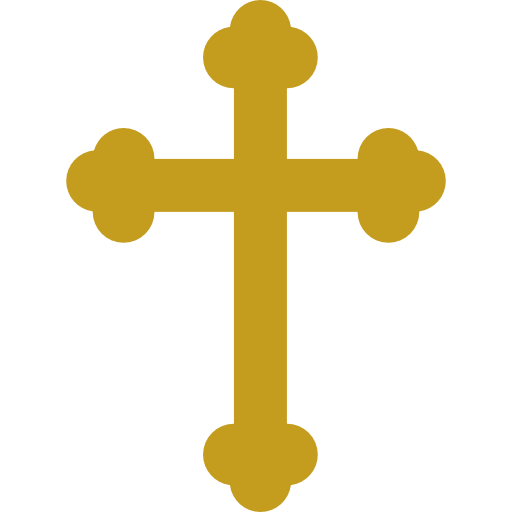
\includegraphics[scale=0.2]{assets/cross.png}\quad
  \textit{Augusta Rainha}
}
\fancyfoot[RO,RE]{\thepage}

\begin{document}

\title{\textbf{Augusta Rainha dos Céus}}
\date{}
\maketitle

\section{Oração Augusta Rainha dos Céus}

Antes de começarmos, queremos recordar um fato histórico essencial, que decora e justifica toda a importância desta oração, que foi revelada ao Padre Louis-Édouard Cestac em 13 de janeiro de 1864 pela Virgem Maria.

Em sua aparição em La Salette, em 1846, Nossa Senhora anunciou a Mélanie Calvat que:  
\say{No ano de 1864, Lúcifer, com um grande número de demônios, será solto do inferno; eles abolirão gradualmente a fé, até mesmo nas pessoas consagradas a Deus; eles as cegarão de tal maneira que, a menos que tenham uma graça especial, essas pessoas tomarão o espírito desses anjos maus; várias comunidades religiosas perderão completamente a fé e perderão muitas almas.} 

Este é o relato da maravilhosa revelação da Santíssima Virgem Maria ao Padre Louis-Édouard Cestac, zeloso servidor da Mãe de Deus, fundador do Convento de Nossa Senhora do Refúgio e da Congregação dos Servos de Maria do Ângulo.

\subsection{A aparição ao Padre}

Foi em 13 de janeiro de 1864 que o Padre Cestac "foi atingido como por um raio de claridade divina".  

Nessa visão, o Venerável Padre acreditava ver os demônios se espalhando pela Terra, causando uma devastação incomensurável.  
Então a Virgem Maria teria dito a ele que os demônios foram libertados no mundo, e que havia chegado a hora de ela ser invocada como Rainha e Soberana dos Anjos, para que lhe pedissem que enviasse as legiões celestiais para lutar e destruir os poderes do inferno.

Surpreso e assustado, o Padre Cestac respondeu:  
“Mas, minha Mãe, Vós que sois tão boa, não podeis mandar os vossos anjos sem precisar que vos peçamos?”

Ele foi ordenado a mandar imprimir esta oração às suas próprias custas e distribuí-la gratuitamente por toda a França, "totalmente livre, proibindo receber qualquer pagamento, direto ou indireto".  
O Padre Cestac mandou imprimir 500.000 cópias.  
A oração foi então recomendada para comunidades religiosas, escolas, famílias cristãs... Rapidamente, foi aprovada pela autoridade eclesiástica de Tarbes, Aire, Tours e Cambrai.

Mas essa oração deveria se espalhar pelo mundo. E assim aconteceu. A oração revelada ao Venerável Padre Cestac se difundiu na Espanha, Alemanha, Itália, Inglaterra e até mesmo no Novo Mundo (América do Norte e América do Sul), sendo traduzida para várias línguas.

O que conferiu a essa oração uma marca eterna e uma alta aprovação foi a autorização suprema do venerado Pontífice, Pai de toda a família cristã.

Para isso, o Venerável Padre Cestac escreveu, logo em 13 de janeiro de 1864, ao Cardeal Villecourt, então Bispo de La Rochelle:  
"É em nome da Divina Mãe, Rainha e Soberana Senhora dos Anjos, que me ajoelho, Eminência, e peço que apresente ao nosso Santíssimo e muito venerado Santo Padre esta pequena oração, da qual envio algumas cópias."

Como resultado, a oração foi submetida à avaliação do Papa, implorando-huma humilde aprovação e bênção.  
Em 17 de fevereiro de 1864, o piedoso Cardeal Villecourt transmitiu ao Padre Cestac a resposta papal do Papa Pio IX, acrescentando:  
"Não há nada que possa ser rejeitado em orações que tendam a reverter os desígnios do demônio e frear sua malícia."

Após retomar brevemente a fabulosa história desta oração, voltamos agora a alguns fenômenos extraordinários e sobrenaturais que ocorreram durante sua propagação, que não ocorreu sem grandes dificuldades.

Apesar de todos os ataques e do desencadeamento infernal contra esta oração, nenhum demônio ou servo seu pôde impedir sua difusão pelo mundo.  
Esta oração foi objeto de numerosas e brilhantes autorizações episcopais, além de ser aprovada e recomendada pelo Papa Pio IX.  
Ademais, seus sucessores, Leão XIII e São Pio X, enriqueceram-na com indulgências.

Finalmente, apresentamos esta oração como é conhecida e rezada hoje, mesmo que tenha sofrido pequenas modificações.

Esperamos que esta oração, considerada uma das mais poderosas para combater o demônio e suas influências, seja conhecida, compartilhada e recitada por todos.

\newpage

\section{Oração Augusta Rainha dos Céus}


\begin{verse}
Augusta Rainha dos céus, soberana mestra dos Anjos,\\
Vós que, desde o princípio, recebestes de Deus\\
o poder e a missão de esmagar a cabeça de Satanás,\\
Nós vo-lo pedimos humildemente,\\
Enviai vossas legiões celestes para que,\\
sob vossas ordens, e por vosso poder,\\
Elas persigam os demônios, combatendo-os por toda a parte,\\
Reprimindo-lhes a insolência, e lançando-os no abismo.\\
Quem é como Deus?\\
Ó Mãe de bondade e ternura,\\
Vós sereis sempre o nosso Amor e a nossa esperança.\\
Ó Mãe Divina,\\
Enviai os Santos Anjos para nos defenderem,\\
E repeli para longe de nós o cruel inimigo.\\
Santos Anjos e Arcanjos,\\
Defendei-nos e guardai-nos. Amém.

\end{verse}

\response. \quad Rogai por nós, Santa Mãe de Deus,

\versicle. \quad Para que sejamos dignos das promessas de Cristo. \\

\vfill

\begin{center}
\subsection*{Fontes:}
\underline{\href{https://catholiquedefrance.fr/histoire-de-la-priere-auguste-reine-des-cieux/}{Catholiques de France}}\\
\underline{\href{https://padrepauloricardo.org/blog/aprenda-a-oracao-augusta-rainha-dos-ceus}{Site Padre Paulo Ricardo}}\\

\end{center}


\end{document}
